\documentclass[12pt,letterpaper]{beamer}
\usetheme{Copenhagen}
\usecolortheme{seahorse}
\setbeamertemplate{section in toc}{\inserttocsection}

\usepackage[utf8]{inputenc}
\usepackage{amsmath}
\usepackage{amsfonts}
\usepackage{amssymb}
\usepackage{graphicx}
\graphicspath{ {./images/} }
\usepackage{multirow}
\usepackage{hyperref}
\hypersetup{
    colorlinks=true,
    linkcolor=blue,
    filecolor=magenta,      
    urlcolor=cyan,
    pdftitle={Overleaf Example},
    pdfpagemode=FullScreen,
}
\usepackage{minted}

\title[Robotics I]
{ENGR 3421: ROBOTICS I}
\subtitle{RaspberryPi Camera}

\author[Zhang, Lin]
{Dr. Lin Zhang}
\institute[UCA] % (optional)
{
  Department of Physics and Astronomy\\
  University of Central Arkansas
}
\date[Robotics1 2021] % (optional)
{September 16, 2021}
\logo{
\includegraphics[height=1cm]{../images/uca_bear_logo.png}}


%End of title page configuration block
%------------------------------------------------------------

%------------------------------------------------------------
%The next block of commands puts the table of contents at the beginning of each section and highlights the current section:

\AtBeginSection[]
{
  \begin{frame}
    \frametitle{Outline}
    \tableofcontents[currentsection]
  \end{frame}
}
%------------------------------------------------------------

\begin{document}

%The next statement creates the title page.
\frame{\titlepage}

%---------------------------------------------------------
%This block of code is for the table of contents after the title page
\begin{frame}
\frametitle{Outline}
\tableofcontents
\end{frame}
%---------------------------------------------------------

\section{RaspberryPi Camera}

\begin{frame}{RaspberryPi Camera}
    \begin{columns}
        \column{0.5\textwidth}
        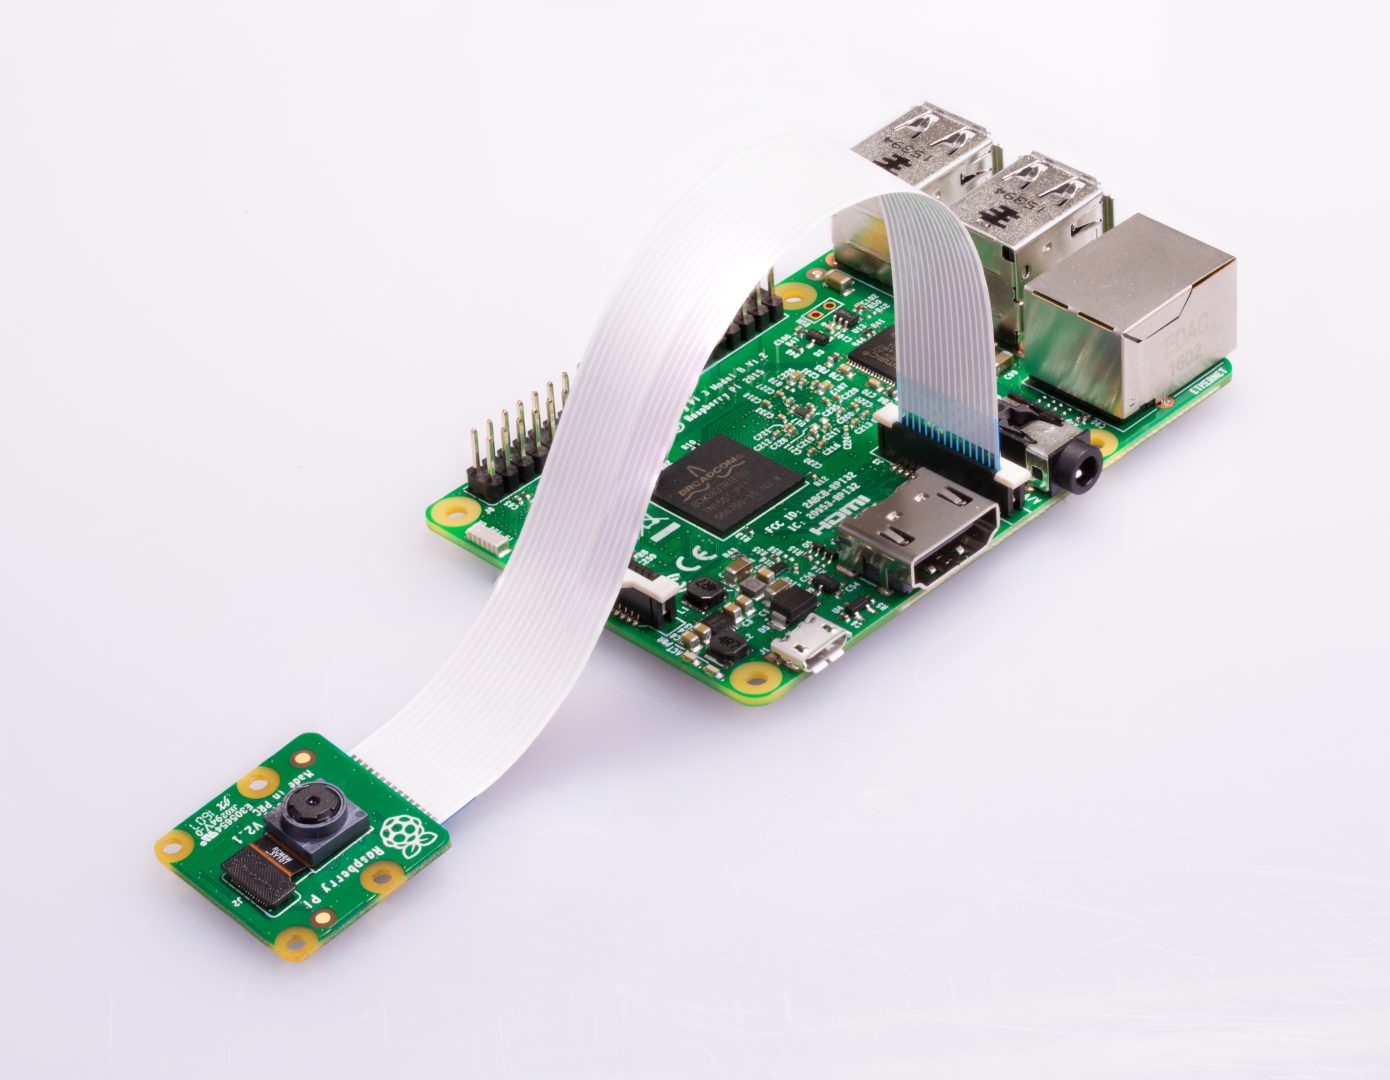
\includegraphics[width=0.9\textwidth]{picamera_attached}

        \column{0.5\textwidth}
        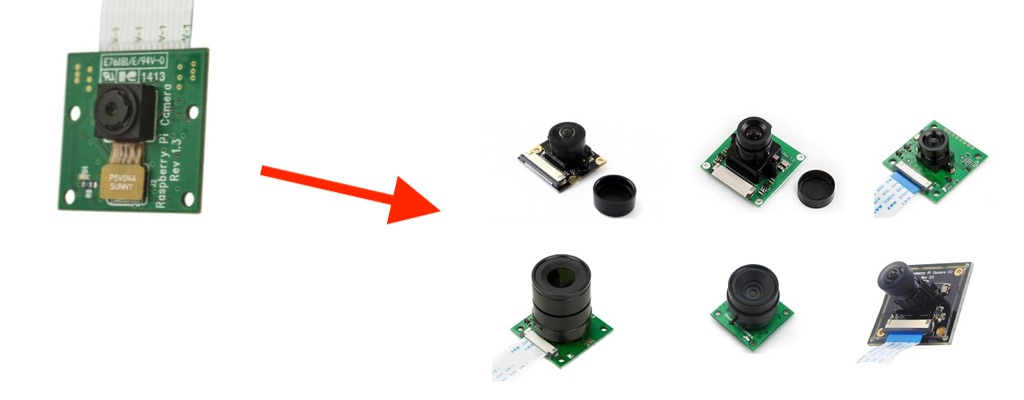
\includegraphics[width=0.9\textwidth]{camera_variations}
    \end{columns}
\end{frame}

\begin{frame}[fragile]
    \frametitle{picamera Library}
    Refer to the \href{https://projects.raspberrypi.org/en/projects/getting-started-with-picamera}{tutorial} and the official \href{https://picamera.readthedocs.io/en/release-1.13/}{documents}.
    \rule{\textwidth}{1pt}   
    \scriptsize
    \begin{minted}{python}
        from picamera import PiCamera
        from time import sleep

        camera = PiCamera()

        camera.start_preview()
        sleep(5)
        camera.stop_preview()
    \end{minted}
    \rule{\textwidth}{1pt}   
\end{frame}

\section{OpenCV}

\begin{frame}{OpenCV}
    \href{https://opencv.org/}{OpenCV} (Open Source Computer Vision Library) is an open source computer vision and machine learning software library. 
    OpenCV was built to provide a common infrastructure for computer vision applications and to accelerate the use of machine perception in the commercial products.
    \centering
    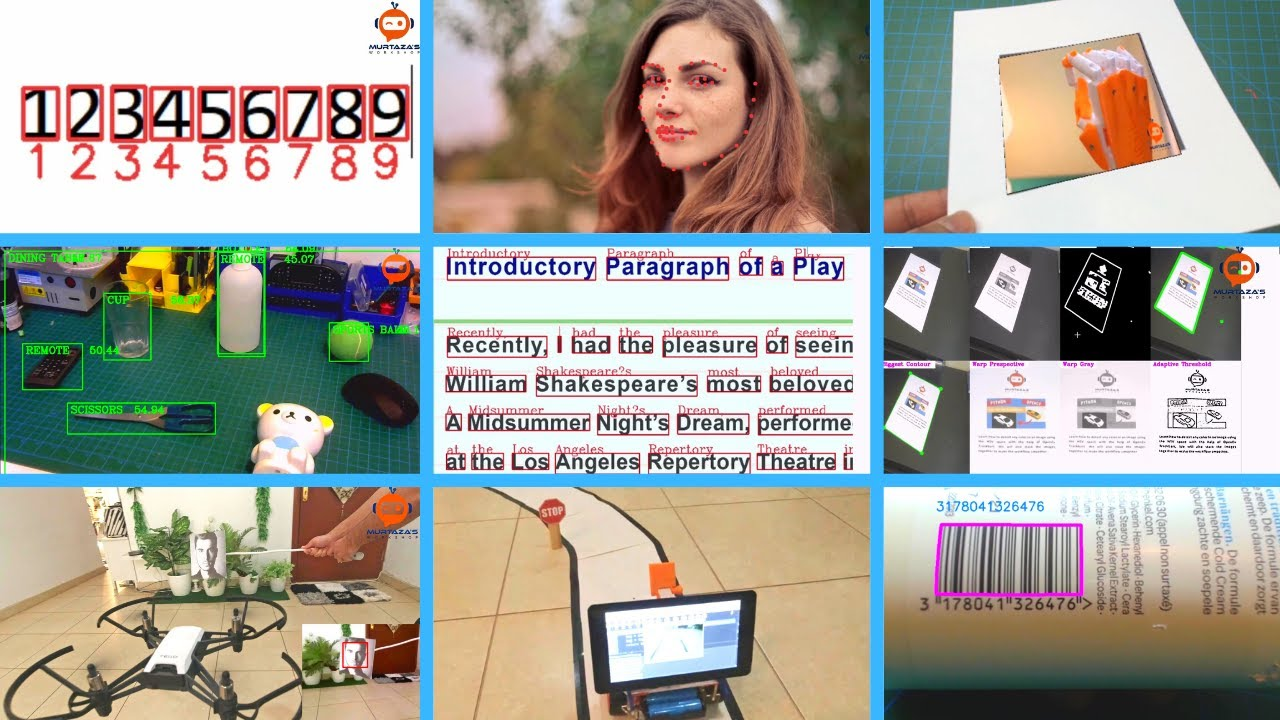
\includegraphics[width=0.7\textwidth]{opencv_projects}
\end{frame}

\begin{frame}[fragile]
    \frametitle{OpenCV Video Capturing}
    \rule{\textwidth}{1pt}   
    {\scriptsize
    \begin{minted}{python} 
        import cv2

        cap = cv2.VideoCapture(0)
        cap.set(cv2.CAP_PROP_FRAME_WIDTH,640)
        cap.set(cv2.CAP_PROP_FRAME_HEIGHT,480)
        cap.set(cv2.CAP_PROP_FPS, 24)
        for i in range(1000):
            ret, img = cap.read()
            # show the frame
            cv2.imshow("Frame", img)
            key = cv2.waitKey(1) & 0xFF
            # if the `q` key was pressed, break from the loop
            if key == ord("q"):
                break
        cap.release()
        cv2.destroyAllWindows()
    \end{minted} 
}
    \rule{\textwidth}{1pt}   
\end{frame}


\end{document}

